\section{Exceptions}

\begin{definition}[\textit{Interrupt}]
    An interrupt is an external or internal event that necessitates processing by another system program.
\end{definition}
Interrupts, typically unexpected or infrequent from the program's perspective, can arise from various causes.
Exceptions can be categorized as follows:
\begin{itemize}
    \item [a.]\textit{Synchronous}: events from devices external to the CPU and memory, manageable after the current instruction completes, making them easier to handle.
    \item [b.]\textit{Asynchronous}: events initiated by the current instruction.
    \item [a.]\textit{User requested}: predictable and treated similarly to exceptions, using the same mechanisms for saving and restoring state; handled after instruction completion.
    \item [b.]\textit{Coerced}: arise from hardware events beyond the program's control.
    \item [a.]\textit{User maskable}: the mask determines whether the hardware responds to the exception.
    \item [b.]\textit{User non-maskable}: exceptions that cannot be ignored by the user.
    \item [a.]\textit{Within instructions}: typically synchronous as the instruction initiates the exception, requiring the instruction to halt and restart.
    \item [b.]\textit{Between instructions}: asynchronous exceptions arising from critical situations, often leading to program termination.
    \item [a.]\textit{Terminate}: program execution always halts after the interrupt.
    \item [b.]\textit{Resume}: program execution continues after the interrupt.
\end{itemize}

\paragraph*{Asynchronous interrupt}
In the case of an asynchronous interrupt, an I/O device signals the need for attention by activating a prioritized interrupt request line.
When the processor decides to handle the interrupt, it completes all instructions before the current one, saves the PC in a dedicated register called the Exception Program Counter (EPC), disables all interrupts, and then transfers control to a specified interrupt handler operating in kernel mode.
Before enabling interrupts to accommodate nested interrupts, the interrupt handler:
\begin{itemize}
    \item Saves the PC into general-purpose registers
    \item Temporarily blocks further interrupts until the PC is saved
    \item Retrieves information about the interrupt cause from a designated status register.
\end{itemize}
The interrupt handler then uses a specialized indirect jump instruction called Return-From-Exception (RFE) to: enable interrupts, restore the processor to user mode, and reinstate hardware status and control state

\paragraph*{Synchronous interrupt}
A synchronous interrupt, also known as an exception, is triggered by a specific instruction. 
Typically, the instruction cannot finish execution and must be restarted after handling the exception, necessitating the undoing of one or more partially executed instructions. 
However, in the case of a system call trap, the instruction is considered fully executed, involving a special jump instruction that transitions to privileged kernel mode.

\subsection{Precise interrupt}
\begin{definition}[\textit{Precise interrupt}]
    An interrupt or exception is deemed precise when a singular instruction (or interrupt point) exists at which all preceding instructions have finalized their state, and no subsequent instructions, including the interrupting instruction, have altered any state.
\end{definition}
This implies that execution can effectively resume from the interrupt point, yielding the correct outcome.
Precise interrupts are desirable for several reasons:
\begin{itemize}
    \item They facilitate the restart of various interrupt and exception types
    \item They simplify the process of determining the exact cause of the interruption
\end{itemize}
While restartability doesn't mandate preciseness, it significantly enhances the ease of restarting. 
Preciseness notably streamlines the task for the operating system, requiring less state to be preserved when unloading processes and allowing for quicker restarts.

\subsection{Exceptions in pipeline}
Exceptions can arise at various stages within the pipeline. 
The recommended approach for handling these interrupts is to minimize pipeline interruption as much as possible.
\begin{figure}[H]
    \centering
    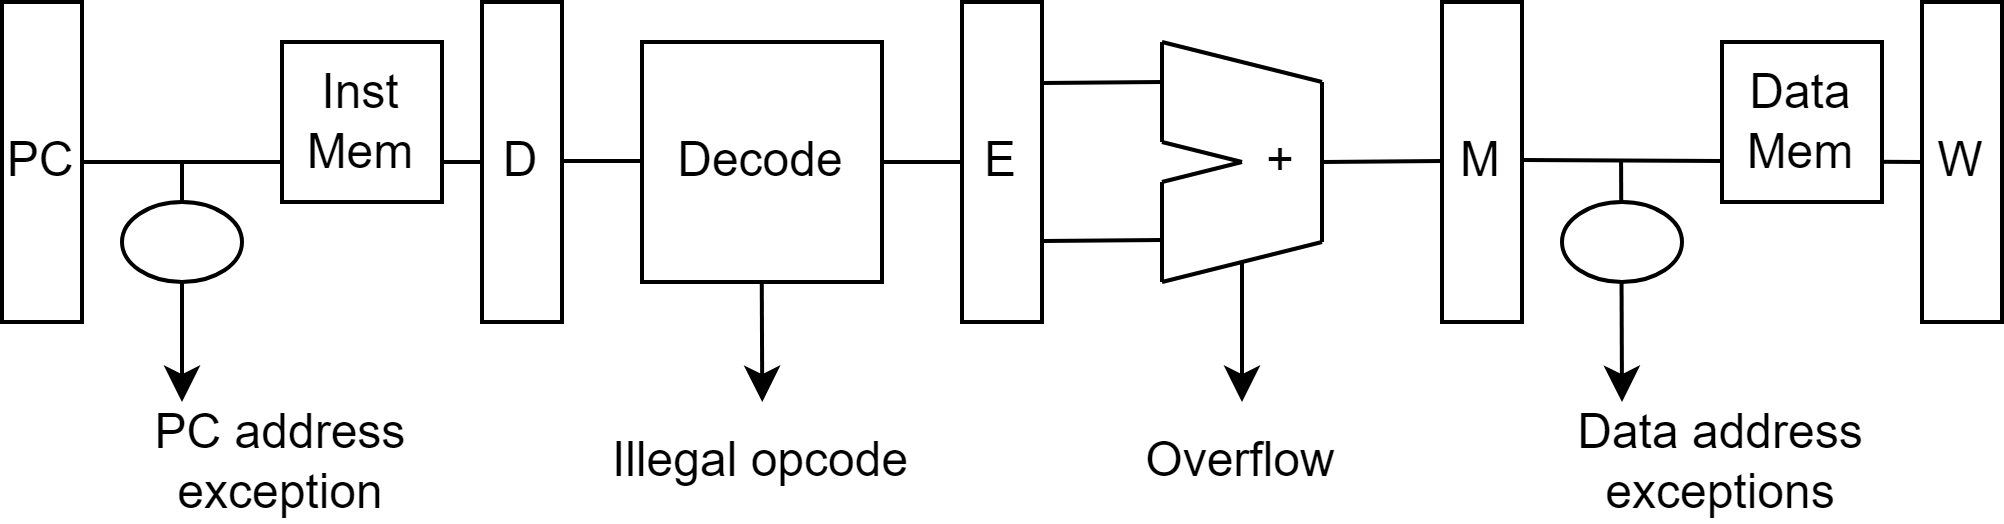
\includegraphics[width=0.75\linewidth]{images/5s.png}
    \caption{Exception origins}
\end{figure}
To manage this, instructions in the pipeline can be tagged to indicate whether they cause exceptions. 
This tagging process waits until the memory stage concludes before flagging an exception. 
Interrupts are then represented as no-operation (nop) placeholders inserted into the pipeline instead of regular instructions.

In cases where a nop is flushed, it is assumed that the interrupt condition persists. 
Managing interrupt conditions can be complex due to requirements such as switching to supervisor mode and saving one or more PCs.

Optimizing the instruction fetch to start fetching instructions from the interrupt vector can also be challenging due to these complexities.
\begin{figure}[H]
    \centering
    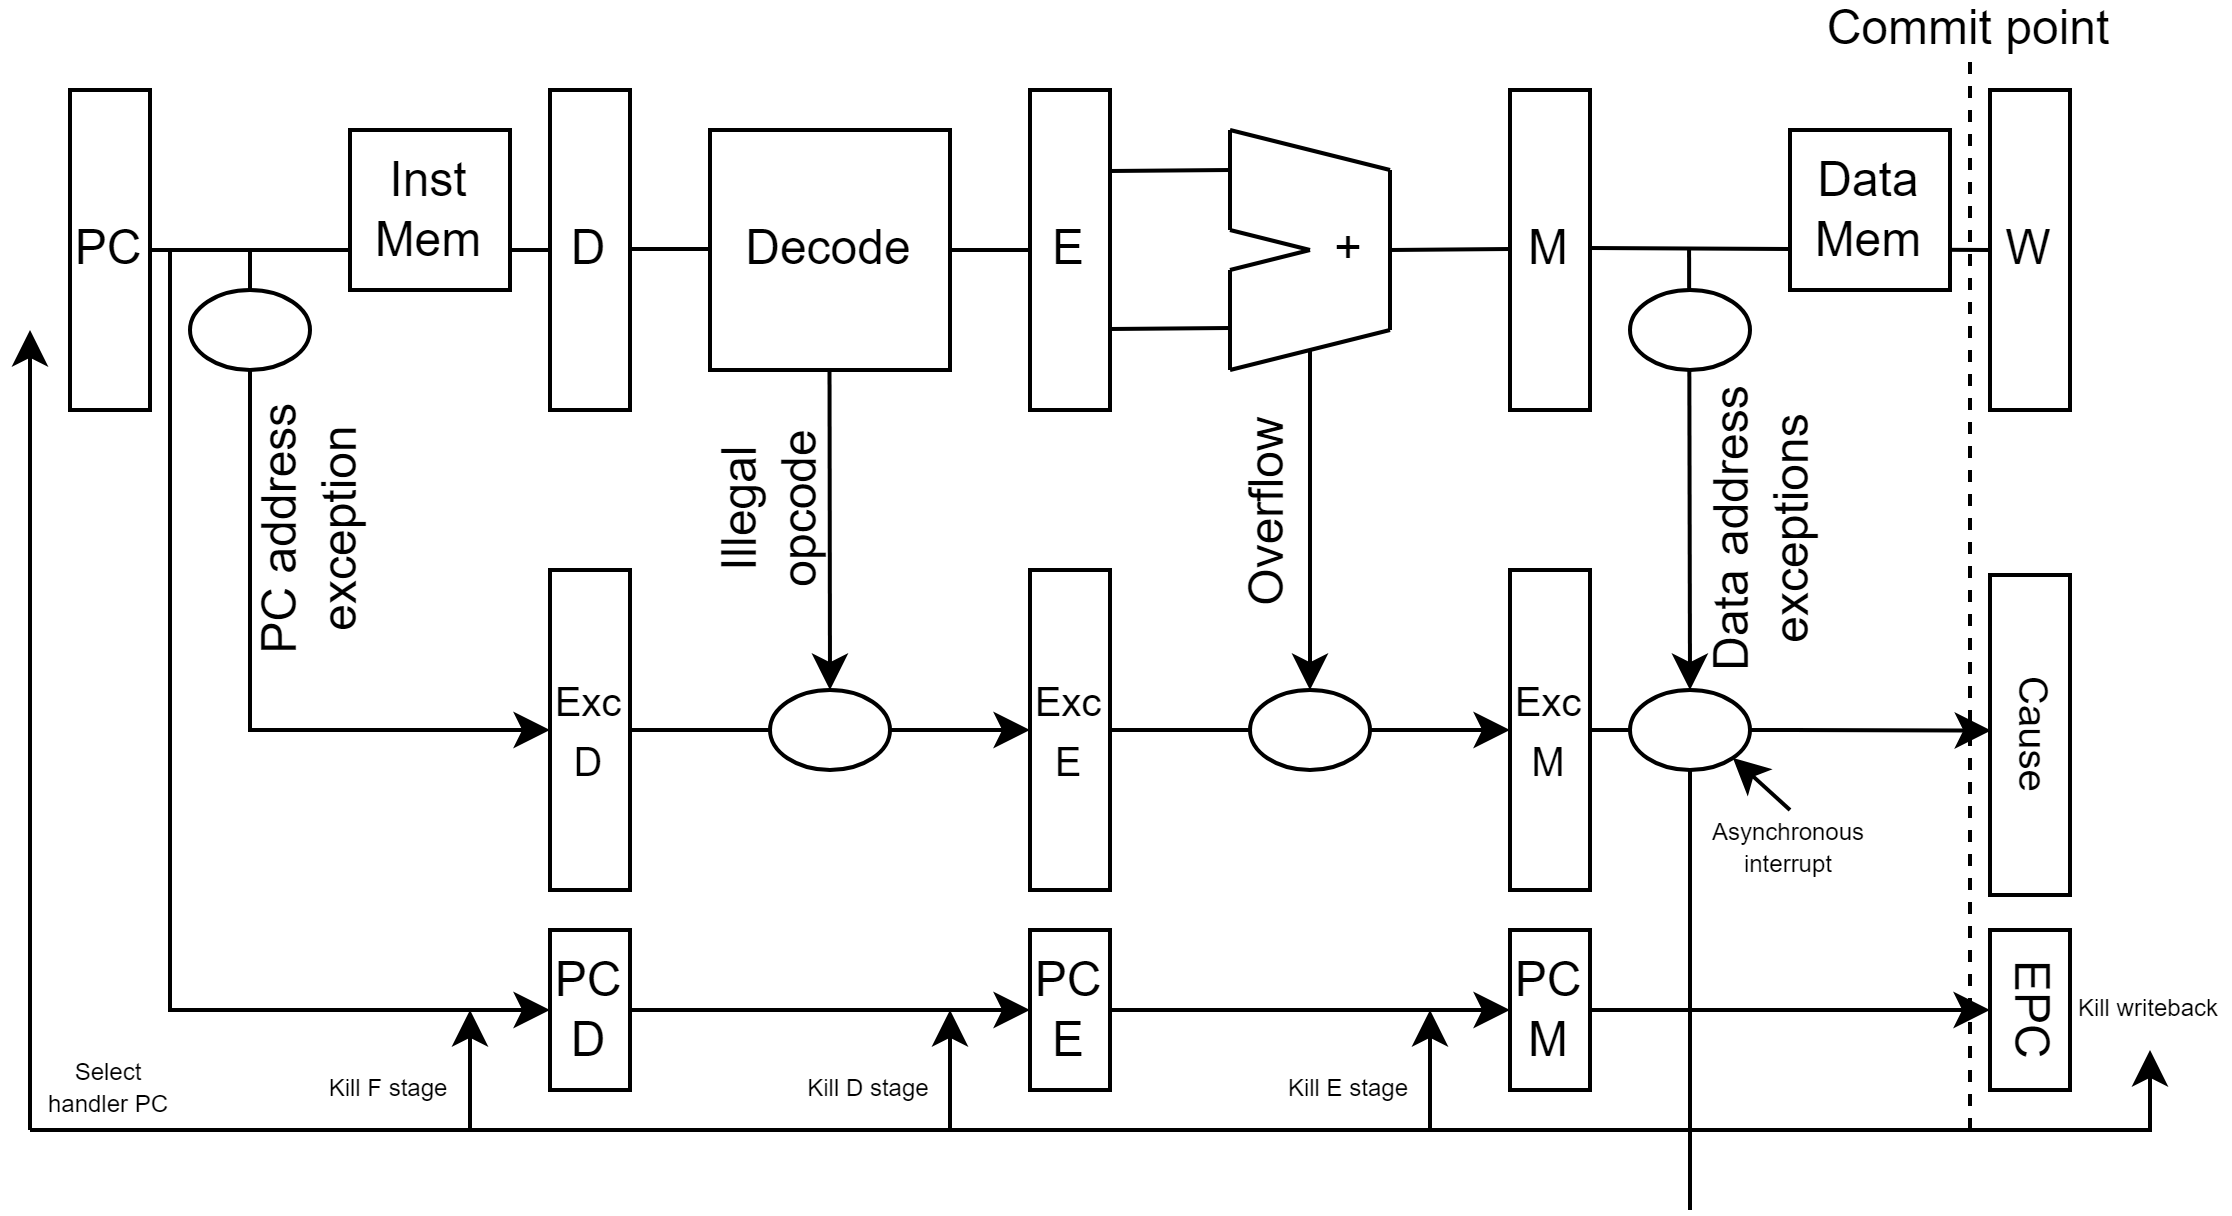
\includegraphics[width=0.75\linewidth]{images/5s2.png}
    \caption{Exception handling}
\end{figure}
Exception flags are maintained within the pipeline until reaching the commit point. 
Exceptions occurring in earlier pipeline stages take precedence over later ones for a particular instruction. 
External interrupts are injected at the commit point, overriding any other exceptions present.

If an exception occurs at the commit point, the cause and EPC registers are updated, all pipeline stages are terminated, and the handler PC is injected into the fetch stage.

\subsection{Exceptions prediction}
Methods to anticipate exceptions include:
\begin{itemize}
    \item \textit{Prediction mechanism}: given the infrequent occurrence of exceptions, a straightforward prediction of no exceptions yields high accuracy.
    \item \textit{Verification of prediction mechanism}: exceptions are identified at the conclusion of the instruction execution pipeline, utilizing specialized hardware tailored for different exception types.
    \item \textit{Recovery mechanism}: architectural state is exclusively written at the commit point, allowing the discarding of partially executed instructions after an exception.
        Following the exception, the pipeline is flushed, and the exception handler is initiated.
    \item \textit{Bypassing}: bypassing facilitates the utilization of uncommitted instruction outcomes by subsequent instructions.
\end{itemize}